%Erzeugt mit dem LaTeX-Generator: http://latex.sehnot.de

%Schriftgröße, Layout, Papierformat, Art des Dokumentes
\documentclass[12pt,oneside,a4paper]{scrbook}

%Einstellungen der Seitenränder
\usepackage[left=3cm,right=4cm,top=1cm,bottom=1cm,includeheadfoot]{geometry}

%neue Rechtschreibung
\usepackage{ngerman}

%Umlaute ermöglichen
\usepackage[utf8]{inputenc}

%Kopf- und Fußzeile
\usepackage{fancyhdr}
\pagestyle{fancy}
\fancyhf{}

%Paket Longtable
\usepackage{longtable}

%Kopfzeile rechts bzw. außen
\fancyhead[R]{\today}
%Linie oben
\renewcommand{\headrulewidth}{0.5pt}

%Fußzeile mittig
\fancyfoot[C]{\thepage}
%Linie unten
\renewcommand{\footrulewidth}{0.5pt}

%Bildpaket
\usepackage{graphicx}

%Verlinkung
\usepackage[unicode]{hyperref} 

\usepackage{url}       % URLs im Literaturverzeichnis

\title{Architektur von Datenbanksystemen \\ Praktikumsbericht 1}
\author{Benedikt Kappes \\ Tuan-Si Tran}

\makeatletter
\renewcommand\chapter{\par%
  \thispagestyle{plain}%
  \global\@topnum\z@
  \@afterindentfalse
  \secdef\@chapter\@schapter}
\makeatother


\begin{document}
\maketitle
\chapter{Einleitung}
Im ersten Praktikum ist das Ziel die IBM DB2 - Datenbank kennenzulernen. Die Installation des Datenbanksystems auf Linux ist schon als VMWare-Image vorhanden, welche auch in diesem Praktikum benutzt wird. Dabei werden in diesem Team sowohl ein Laptop mit mechanischer Festplatte als auch ein Laptop mit SSD-Platte eingesetzt.\\

Im ersten Schritt werden Überlegungen im Vorfeld zur Größe der zuschreibenden Daten in die Datenbank gemacht. Als nächstes werden die Datenbank erzeugt und die Daten mit einer Java-Anwendung und der Benutzung des JDBC-Treibers in die Datenbank eingetragen. Von Interesse sind hierbei Zeitdauer und die tatsächliche Größe der Datenbank bzw. der geschriebenen Daten. Im letzten Abschnitt werden die
\chapter{Vorbereitung}
Im Laufe des erstens Praktikums muss die Datenbank mit Testdaten befüllt werden. Im Vorfeld soll dabei die Größe der Datenbank geschätzt werden, nachdem die Daten erzeugt und gespeichert worden sind. 
Dabei wurde mit Hilfe der Tabelle (siehe Anhang \ref{app:01}) die Größe eines Datensatzes ermittelt und mit der Anzahl der zu schreibenden Datensätze multipliziert.\\

Die folgende Auflistung zeigt die Hochrechnung für die drei Tabellen \texttt{Kunde}, \texttt{Produkt} und \texttt{Bestellung} an (siehe Tabelle \ref{tbl:size_of_data}).
\begin{longtable}{|l|l|r|r|} \hline
%\begin{tabular}{|l|l|r|l|} 
\multicolumn{4}{|l|}{ \textbf{Kunde}}\\
Spaltenname & Typ & Byte Count & \\
\hline 
KNR & Integer & 4 Byte & \\
KNAME & Char & 20 Byte & \\ 
KVORNAME & Char & 15 Byte &\\ \hline
\multicolumn{2}{|r}{} & 100 x 39 Byte & = 3 900 Byte \\ \hline

\multicolumn{4}{|l|}{ \textbf{Produkt}}\\
Spaltenname & Typ & Byte Count &\\
\hline 
PID & Integer & 4 Byte & \\
PRODUKTNAME & Char & 20 Byte & \\ 
PREIS & Decimal(6,2) & 4 Byte & \\ \hline
\multicolumn{2}{|r}{} & 1000 x 28 Byte & = 28 000 Byte \\ \hline

\multicolumn{4}{|l|}{ \textbf{Bestellung}}\\
Spaltenname & Typ & Byte Count &\\ \hline 
BID & Integer & 4 Byte & \\
KNR & Integer & 4 Byte & \\ 
PID & Integer & 4 Byte & \\ 
DATUM & Date & 4 Byte & \\ 
STATUS & Smallint & 2 Byte & \\ \hline
\multicolumn{2}{|r}{} & 750 000 x 18 Byte & = 13 500 000 Byte \\ \hline
\multicolumn{3}{|r}{Summe} & = 13 531 900 Byte \\ \hline
%\end{tabular}
\caption{Berechnung der Größe der Testdaten}
\label{tbl:size_of_data}
\end{longtable}
Als Gesamtgröße für die reine Datenmenge wird in etwa 13,5 MB angenommen (bei 1000Byte = 1 KByte). 

\section*{Fremdschlüsselindex}
Wird der Fremdschlüsselindex nicht angelegt bei der Erzeugung der Tabelle, sollte das Eintragen der Daten schneller gehen. Nach unseren Erwartungen sollte das nachträgliche Erzeugen des Fremdschlüsselindexes für die Tabelle \texttt{Bestellung} einige Zeit in Anspruch nehmen.
\chapter{Durchführung}
Über das Befehlszeilenfenster wurde die Datenbank \texttt{ArchDBS} erzeugt und den \textit{Footprint} der leeren Datenbank ermittelt. Danach wurde das Java-Konsolen-programm erstellt, das 100 Kundentupel, 1000 Produkttupel und 750 000 Bestellungen in die Datenbank eingetragen hat. Dabei wurde die Zeit gemessen, die für die Erstellung der 751100 Tupel benötigt wurden. Damit die Erzeugung der Testdaten performant ablaufen konnte, wurde \texttt{autocommit} auf \texttt{false} gesetzt und \texttt{PreparedStatements} verwendet. Ebenso war es nötig, die maximale Größe der Logdateien (\texttt{LOGPRIMARY} oder \texttt{LOGSECOND}) zu erhöhen, damit die Erzeugung der 750000 Bestellungen auch mitgeloggt werden können. Die Größe der Datenbank wurde erneut ermittelt und mit dem Startwert verglichen.\\

Im nächsten Schritt wurde eine zweite Datenbank mit den entsprechenden Tabellen angelegt, wobei auf Foreign-Keys-Indexe verzichtet worden sind. Erneut wurde die Zeit gemessen und mit dem Wert aus der vorherigen Messung verglichen. Als letztes wurden die Fremdschlüsselindexe über die gefüllten Tabellen erzeugt. 
\chapter{Ergebnisse und Auswertung}
\section{Datenbankgröße}
Der gemessene \texttt{Footprint} unserer leeren Datenbank \texttt{ArchDBS} war 128 MB. Bei genauerer Betrachtung setzt sich die leere Datenbank wie folgt zusammen:\\

--ToDo Table pagesize--\\

Die Seitengröße beträgt für alle drei Tablespaces 4096 Byte.\\

Nach Abruf der Informationen mittels \texttt{list tablespaces show detail} wuchs die Größe der Datenbank allerdings auf 160 MB an. Gründe dafür könnten der Verwaltungsaufwand der Datenbank zur Ermittlung der Tabellendetails sein.\\

Nach der Erzeugung der Testdaten war die Datenbank 192 MB groß. Unsere errechnete Größe lag allerdings bei 183 MB (160 MB + 13.5 MB). Der Fehler beträgt somit unter fünf Prozent. Die Differenz ist hat (hauptsächlich) zwei Ursachen, welche daraus resultieren, dass wir lediglich die genaue Größe der reinen Datenmenge berechnet haben, aber nicht den Overhead eingerechnet haben. Zum einen werden noch die drei Indexe für \texttt{Kunde}, \texttt{Produkt} und \texttt{Bestellung} (mit 750000 Datensätzen) in der Datenbank angelegt, zum anderen werden auch die Seiten nicht zu genau 100 Prozent befüllt. Wenn der Datensatz nicht mehr auf eine Seite passt, wird der freie Restspeicherplatz leer gelassen und die nächste Seite erzeugt. Dadurch beanspruchen die Daten insgesamt mehr Speicherplatz als in unserer Rechnung.\\

\section{Zeitliche Messungen}
Folgende Tabelle stellt die gemessenen Werte dar:\\
--ToDo Tabelle mit Werten--\\

In dieser Tabelle ist zu sehen, dass das Eintragen in die Tabellen der Datenbank \texttt{ArchDBS} wesentlich länger dauert.
\chapter{Zusammenfassung}

\newpage
\chapter{Anhang}
\section{Byte-Count der Datentypen}
\begin{figure}[htbp]
\centering
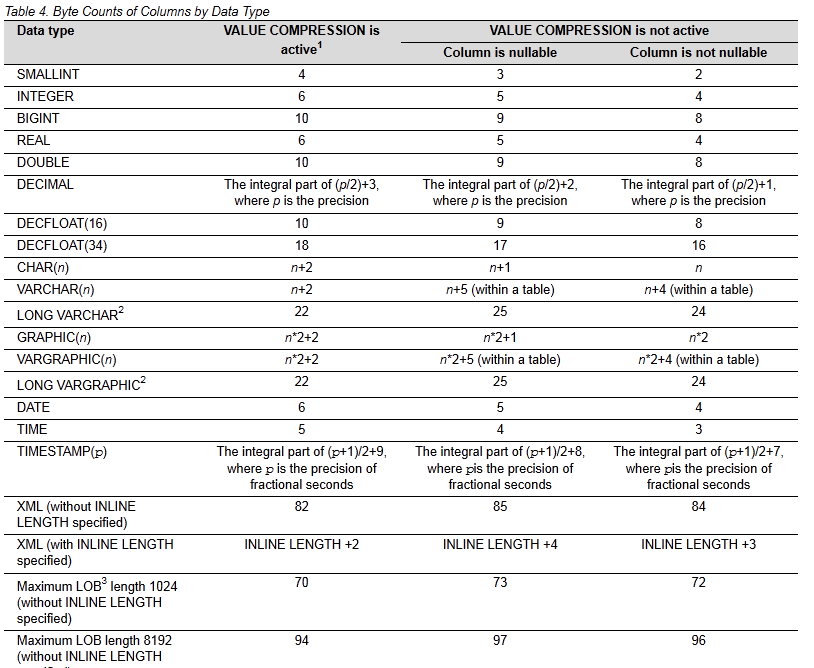
\includegraphics[scale=2.0]{images/01_byte_count.png}%
\caption{Angaben zum Byte-Count, vgl. \cite{IBM-2011a}}%
\label{app:01}
\end{figure}

\newpage
\begin{thebibliography}{-----------}
\bibitem[IBM-2011a]{IBM-2011a} IBM: {\textit{DB2 Solution Information Center}} URL: \url{http://publib.boulder.ibm.com/infocenter/db2luw/v9r7/index.jsp?topic=/com.ibm.db2.luw.sql.ref.doc/doc/r0000927.html}, zuletzt besucht am 20.10.2011


\end{thebibliography}
\end{document}